\documentclass[10pt,twocolumn,letterpaper]{article}

\usepackage{algorithmicx}
\usepackage{algorithm}
\usepackage{booktabs}
\usepackage{cvpr}
\usepackage{graphicx}
\usepackage{algpseudocode}
\usepackage{booktabs}
\usepackage{hyperref}

\renewcommand{\algorithmicrequire}{\textbf{Input:}}
\renewcommand{\algorithmicensure}{\textbf{Output:}}
\renewcommand{\thefootnote}{$\star$}

\cvprfinalcopy % *** Uncomment this line for the final submission

\usepackage{footmisc} % Daggers for author notes
\DefineFNsymbols{mySymbols}{{\ensuremath\dagger}{\ensuremath\ddagger}\S\P
   *{**}{\ensuremath{\dagger\dagger}}{\ensuremath{\ddagger\ddagger}}}
\setfnsymbol{mySymbols}

% Pages are numbered in submission mode, and unnumbered in camera-ready
%\ifcvprfinal\pagestyle{empty}\fi
\setcounter{page}{1}
\begin{document}

%%%%%%%%% TITLE
\title{Methods for handling missing and categorical data for classification with neural
networks$^\star$}

\author{
    Jason Poulos\thanks{\href{mailto:poulos@berkeley.edu}{\nolinkurl{poulos@berkeley.edu}}. SID: 24993379.}
    \hspace{10mm}
    Rafael Valle\thanks{\href{mailto:rafaelvalle@berkeley.com}{\nolinkurl{rafaelvalle@berkeley.com}}. SID: 24090989.}
    \vspace{15mm}
}

\maketitle
%\thispagestyle{empty}

%%%%%%%%% ABSTRACT
\begin{abstract}
Abstract here...
\end{abstract}

\footnotetext[1]{The video presentation can be viewed at \url{youtube.com/foo}.}

%\linenumbers

%% main text
\section{Introduction} \label{section:Intro}

In our project, we plan to investigate techniques for handling missing data and
encoding categorical data such that it is appropriate to neural network
classifiers. \\

Missing data is a common problem in survey data in various domains. Several
techniques for data imputation (i.e., replace missing values with plausible ones) and
direct estimation (i.e., all missing data is analyzed using a maximum likelihood
approach) have been developed ~\cite{de2003prevention}. \\

In the case of categorical variables, which by definition have no direct
representation or computation scheme of the distance between its values,
decision trees can be useful because they do not require distance metrics.
However, their training process is slow given a large enough dataset and they
might not be suitable for problems where the decision boundary between classes
described by a second-order polynomial,\footnote{We note, however, that a
property test can be as complex as the data at hand.} for
example ~\cite{fayyad1996data}. \\

%\section{Related Work}  \label{section:rw}

\section{Methods}

% Explain which methods you are planning to use and why.

\subsection{Techniques for handling missing data}
We divide imputation methods into six groups listed
below ~\cite{batista2003analysis}. Assuming that these techniques are easy to
implement, we would like to compare their efficiency in imputing the missing
values.

\begin{description}
\item[Case substitution] One observation with missing data is replaced with
another non-sampled observation.
\item[Mean or mode imputation] Replace the missing data with the mean or median of
    the feature vector. Since the missing variables in the Adult dataset are
    all categorical, using a numerical approach directly is not appropriate.
\item[One-hot] Create a binary variable to indicate whether or not a specific
    feature is missing. This technique was suggested by Isabelle Guyon.
\item[Hot deck and cold deck] Compute the K-Nearest Neighbors of the
    observation with missing data and assign the mean or median of the K-neighbors
    to the missing data. A similar technique is used in Airbnb's fraud detection
    algorithm.
\item[Prediction Model] Train a single prediction model (e.g., logistic regression,  
    bagging, or boosting) or ensemble of models to predict the missing value. This
    requires correlation amongst features to exist.
\item[Factor analysis] Perform some sort of factorization on the design
    matrix, project the design matrix onto the first two eigen vectors and
    replace the missing values by the values that might be given by the
    projected design matrix.
\end{description}

\subsection{Neural networks for classification with categorical and
quantitative features}  Common techniques for handling categorical data in
neuronal networks include encoding the categorical values into numeric values
or using binary encoding. These techniques, however, have some drawbacks
including unnecessarily increasing model complexity or feature dimensionality
and not preserving the similarity information embedded betweeng categorical
values ~\cite{hsu2006generalizing}.\\

More elaborate techniques include information theoretic measures
~\cite{wang2008categorical}, training separate output units for
each of the allowed combination of values of the categorical independent
variables ~\cite{brouwer2002feed}, and using distance
hierarchies ~\cite{hsu2006generalizing}.

\section{Experiments} \label{section:Experiments}

\subsection{Benchmark data sets}

We plan to experiment with the Adult dataset from the UCI Machine Learning Repository ~\cite{Lichman2013}. The dataset has 48,842 samples ($\mathrm{train}=32,561$ and $\mathrm{test}=1,6281$). The dataset contains 14 features: 6 continuous and 8 categorical. The prediction task is to determine whether a person makes over \$50,000 a year. 24\% of individuals in the training data make more than this amount. \\

Given the results of our experiments and if time permits, we may move to a much larger dataset, such as the 1940 full--count U.S. Census file ~\cite{napp2008, ruggles2010}. The 1940 Census has about 100 million samples and 100 features. 

Table \ref{tab:benchmarks} shows the test error rates obtained by the data set donor ~\cite{kohavi1996}. All error rates were obtained after removing samples with missing values. The error rate to beat is 14.05\%. \\

\begin{table}[htb]
\centering
\begin{tabular}{@{}ll@{}}
\toprule
\textbf{Algorithm}       & \textbf{Error} \\ \midrule
1  C4.5                  & 15.54          \\
2  C4.5-auto             & 14.46          \\
3  C4.5 rules            & 14.94          \\
4  Voted ID3 (0.6)       & 15.64          \\
5  Voted ID3 (0.8)       & 16.47          \\
6  T2                    & 16.84          \\
7  1R                    & 19.54          \\
8  NBTree                & 14.10          \\
9  CN2                   & 16.00          \\
10 HOODG                 & 14.82          \\
11 FSS Naive Bayes       & 14.05          \\
12 IDTM (Decision table) & 14.46          \\
13 Naive-Bayes           & 16.12          \\
14 Nearest-neighbor (1)  & 21.42          \\ \bottomrule
\end{tabular}
\caption{Test set error rates on Adult dataset for various algorithms, obtained after removal of samples with missing values and using the original train/test split. Source: \cite{Lichman2013}.}
\label{tab:benchmarks}
\end{table}

\subsection{Patterns of missing values}

The Adult dataset has 3,620 (7.4\%) samples containing missing values. Missing values occur in three of the categorical features: \textit{Work class}, \textit{Occupation}, and \textit{Native country}. It is unlikely that these values are missing completely at random (MCAR); it is more likely, and much less desirable that the values are not missing at random (MNAR). Since these data originate from a survey, the missing values may be due to respondents unwilling or unable to provide an answer.  \\

Uncovering patterns of missing values in the dataset will help select strategies for imputing missing values. The histogram (left) in Figure \ref{fig:proportion-missing} shows \textit{Work class} and \textit{Occupation} each have about 5.6\% of missing values, and \textit{Native country} has about 1.7\% missing values. The aggregation plot (right) shows 5.5\% of samples are missing values for both \textit{Work class} and \textit{Occupation}. Less than 2\% of samples are missing just \textit{Native country} and less than 1\% are missing all three features.\\

Figure \ref{fig:barplot-missing} shows the frequency of observed categories and missing values for \textit{Work class} and \textit{Occupation}. Each stacked column shows the proportion of missing values in the other feature and \textit{Native country} for each category. The plot shows the missing values are not MCAR: individuals working in the private sector, for instance, are more likely to have missing values than those individuals in other work classes. However, missing values tend to be evenly distributed across occupational categories. 

\begin{figure}[htbp] 
   \centering
   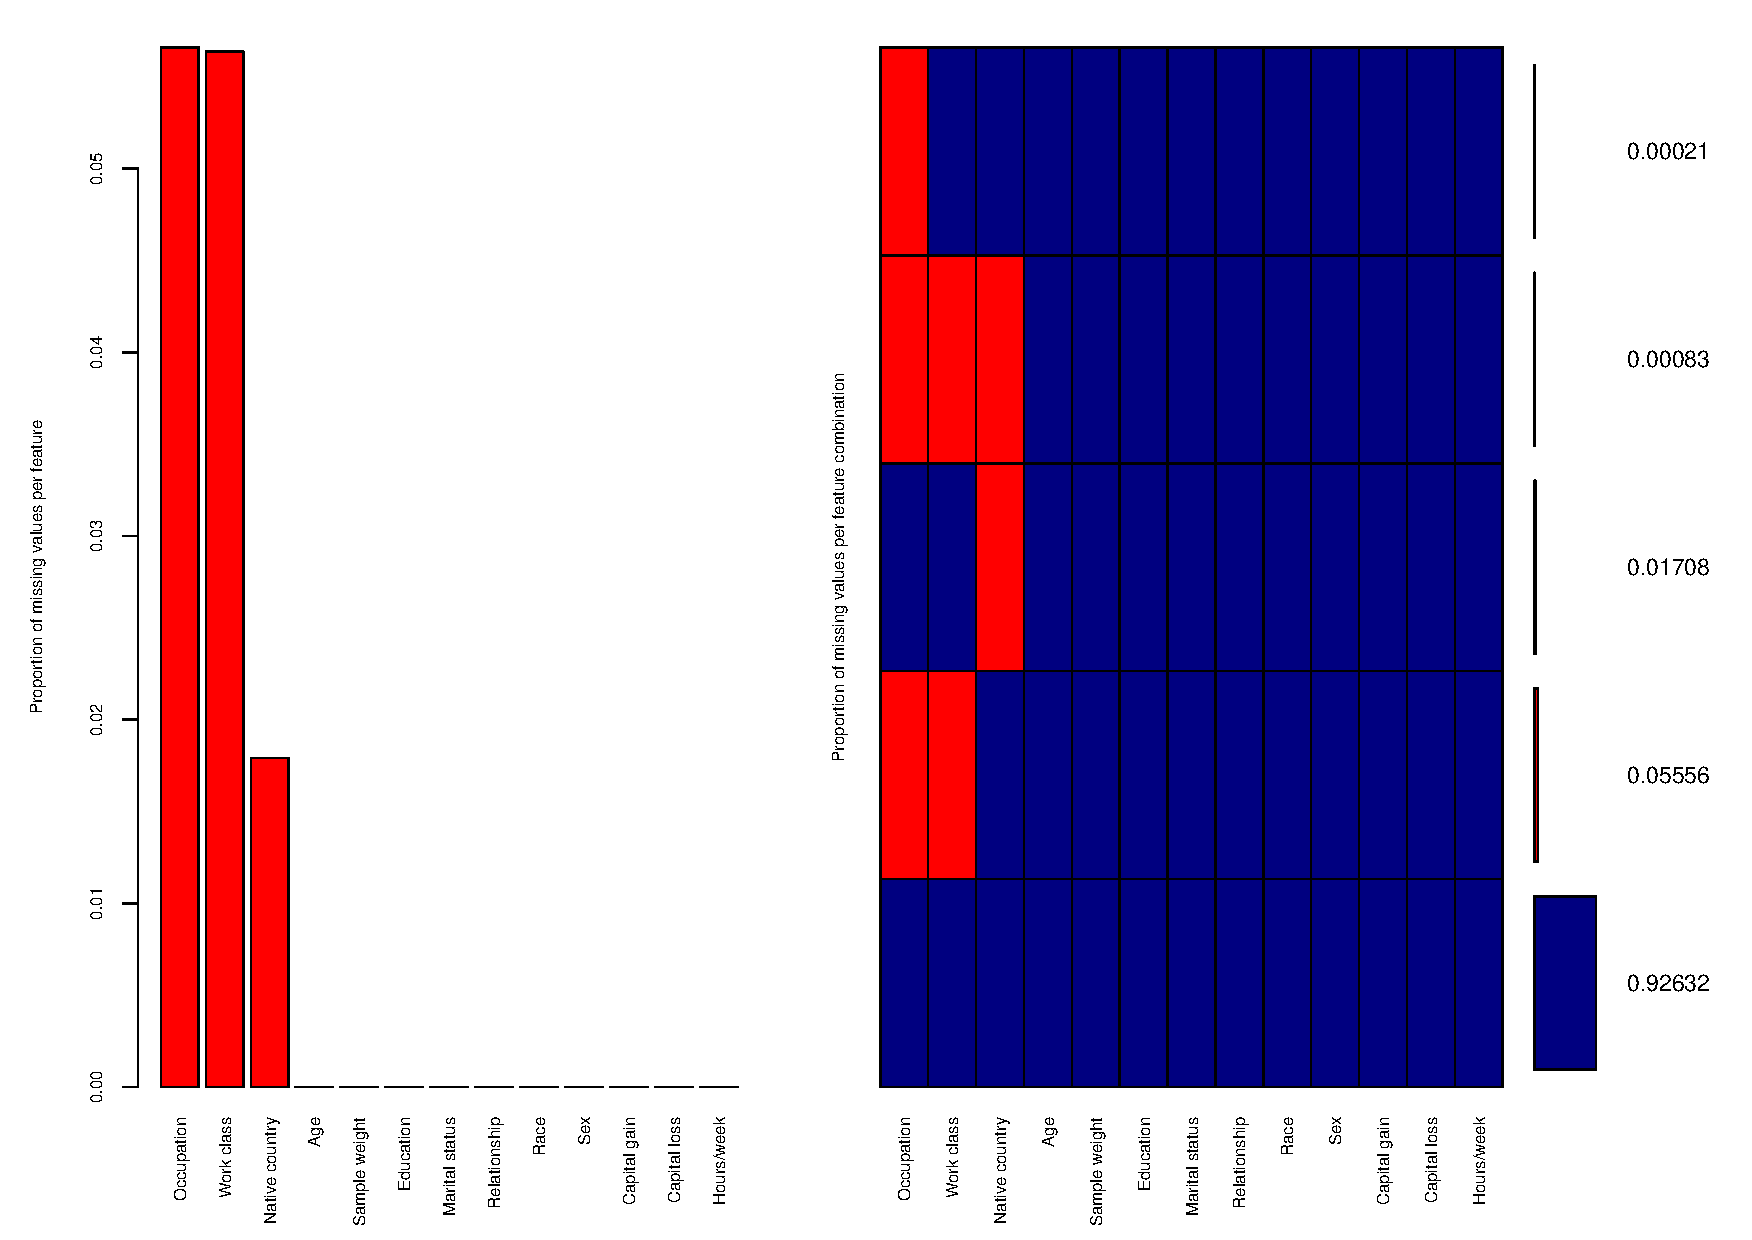
\includegraphics[width=0.5\textwidth]{./figure/proportion-missing.pdf}
   \caption{Histogram of proportion of missing values in each feature (Left) of Adult training set and aggregation plot of all existing combinations of missing and non-missing values in the samples (Right).}
   \label{fig:proportion-missing}
\end{figure}

\begin{figure}[htbp] 
   \centering
   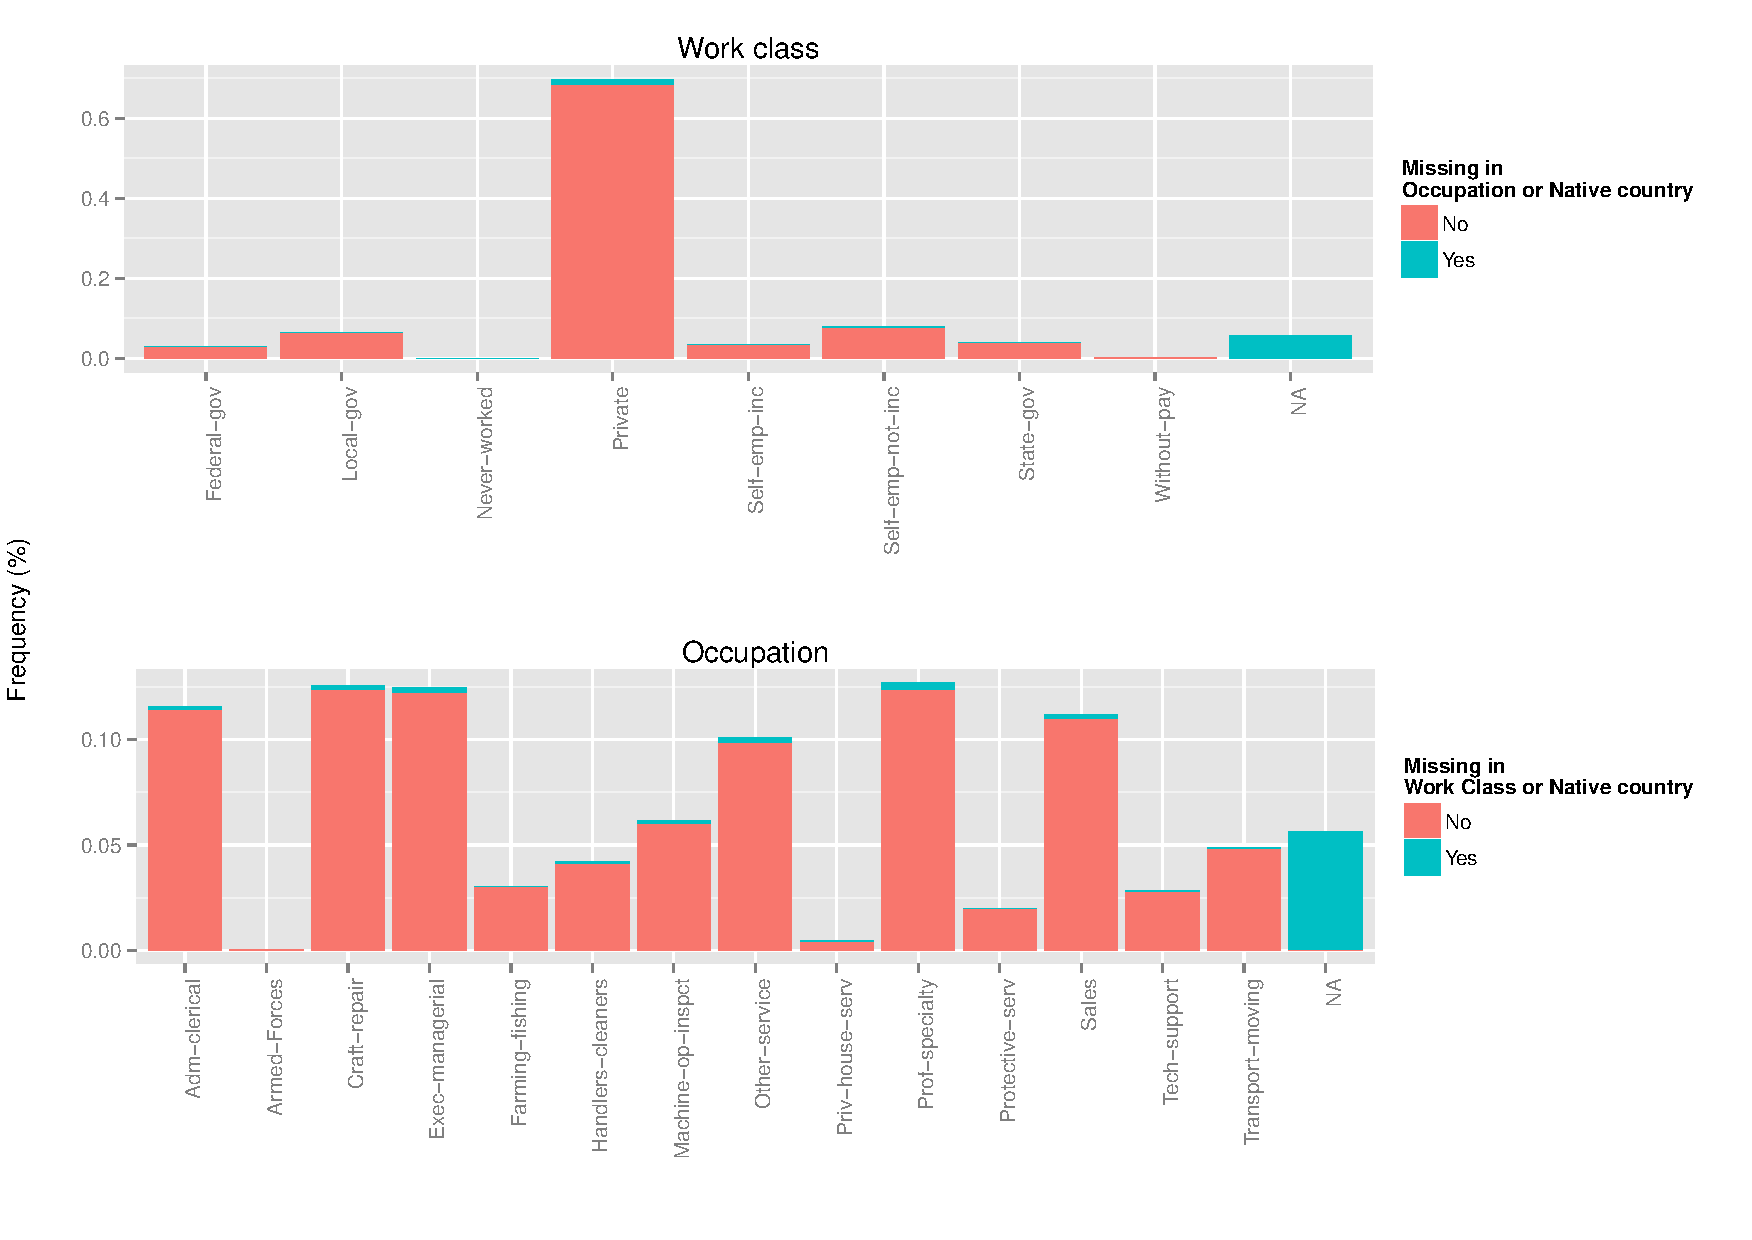
\includegraphics[width=0.5\textwidth]{./figure/barplot-missing.pdf}
   \caption{Barplot of proportion of observed and missing values of \textit{Work class} and \textit{Occupation} in Adult dataset.}
   \label{fig:barplot-missing}
\end{figure}

\section{Conclusions} \label{section:Con}

%\section*{Acknowledgments}

{\small
\bibliographystyle{ieee}
\bibliography{refs}
}

\end{document}
